%% -*- coding: utf-8-unix -*-

\chapter{課題設定}
\label{chap:problem-setting}

 \section{情報システムの構築・運用における課題}
 \label{sec:system-problem}

\ref{sec:pj-purpose}節に示したとおり、情報システムが利用者に提供するサー
ビスは、より速く・柔軟に変化していくことが求められるようになっている。そ
のため、サービス提供者側は、利用者に対して適切なサービス価値が提供できて
いるかどうかを判断していくことが求められる。

システムを構成する各要素がサービスに対する利用者要求の変化に対して柔軟に
変化していくことが求められるが、近年では特にネットワーク部分がサービス変
化の上での迅速性・拡張性の面でのボトルネックになるという状況が発生してい
る。本節ではその理由と課題点について解説する。

% OOD発表資料のp.2-3
% なぜ「ネットワークのテスト」を対象とするのか?
% ネットワークのテストの何が難しいのか?
% これまでネットワークのテストとしてどういったことをおこなっていたのか?

  \subsection{自動化の難しさ}
  \label{sec:difficulty}

ネットワークで自動化がすすまない理由はいくつかあるが、ここではテストの自
動化という観点から、主要な課題について解説する。

    \paragraph{垂直統合の歴史}
歴史的に、ネットワーク機器はベンダごとに異なるOS、異なるAPI(コマンド)を
もち、共通のインタフェースやデータモデルが存在しない。そのため、異なるベ
ンダの機器をつかったネットワークを作ろうとした場合、設定としてはおなじ操
作であっても、異なるAPI(コマンド)で操作する必要がある。

ネットワークに対する操作の自動化はこれまでもおこなわれているが、機器(OS)
ごと、機器の設計上の役割や運用上のオペレーションごとに多数の自動化スクリ
プトを用意する必要があり、複雑かつ汎用性が低い状態になっている。また、複
数のデバイスを操作するうえでは、設定が反映され動作がきりかわるタイミング
などをふまえたうえで、全体のワークフローを考えなければならないという課題
もある。そのため自動化されるのは、シンプルで定型的な処理にとどまることが
多い。\footnote{NW機器を抽象化し統一した方法で異なるAPIの機器を操作可能
にする製品やOSSも存在する(\ref{sec:related-research}節)。しかし、対応し
ていない製品の利用にあたっては、「ドライバ」と呼ばれる操作対象機器のAPI
や取得情報などを機器ごとに別途開発するコストがかかる。APIについては、
Netconf/YANGなどをベースにしたインタフェースやデータモデル標準化の動きは
あるものの、現時点では実装されている機器はまだ少数であり、ベンダ/OSごと
に個別に取り扱う必要がある、という状況である。}

    \paragraph{物理的な位置の操作}
ネットワークは、情報システムの構成要素(計算機リソースなど)の物理的な配置
を抽象化する機能をもつため、ネットワークそれ自体のテストについては、物理
的な配置(場所)を考慮する必要がある。テストされていないネットワークでは、
何らかの問題によりネットワークが通信不可能になる(あるいは一部のネットワー
クで正しく通信ができない)おそれがある。保証されたネットワークの存在を前
提としてよい機能やサービスでは、コネクティビティを前提として作業ができる
ため、ひとつの要素に着目して作業実施・自動化可能なことが多い。しかし、ネッ
トワークのテストはコネクティビティ自体を保証するための作業であり、コネク
ティビティがあることを前提にできない
(\figref{fig:difficulty-of-network-testing})。

 \begin{figure}[h]
  \centering
  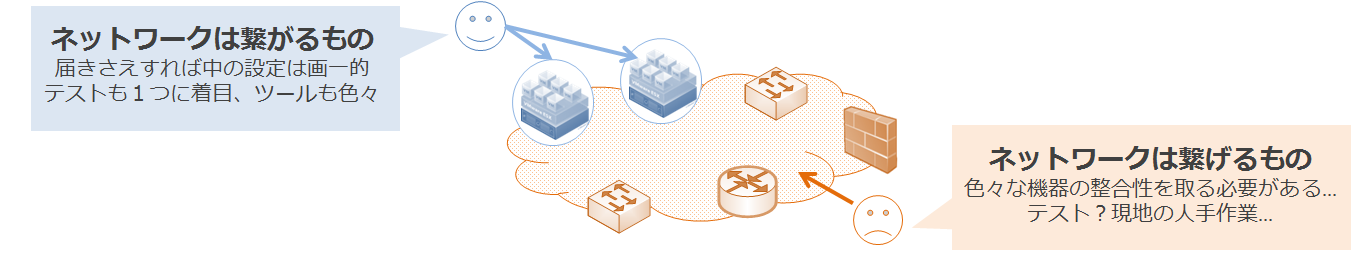
\includegraphics[scale=0.45]{img/difficulty-of-network-testing.png}
  \caption{ネットワークとその他のテストの違い}
  \label{fig:difficulty-of-network-testing}
 \end{figure}

ネットワークの不備あるいはトラブル等により、リモートでのネットワーク機器
へのアクセスが不可能になってしまった場合、機器の現物を直接操作して復旧さ
せなければならない\footnote{こうしたリスクを回避するために、リモートアク
セス用のネットワークとサービス用のネットワークを物理的に分離して設計した
り(out-of-band management network)、機器コンソールをリモートで利用可能に
するための機器(シリアルコンソールサーバ)を導入したりすることがある。しか
し、デバイスの物理的な故障などについてはやはり何らかのかたちで現地・現物
での作業が発生する。}。こうした物理構成上の要求が発生するテスト
\footnote{例えば、リンクダウンなどの物理障害を発生させるケース、ネットワー
ク機器の追加(拡張)・削除といったネットワークの物理構成(トポロジ)を変更す
るケースなど。} は、その「実体を直接操作したい」という要求の性質上、自動
化することが難しい。

    \paragraph{テストケースの組み合わせ爆発}
ネットワークは自律分散制御され、隣接する機器が相互に通信規約の整合性をと
ることで、end-to-end の通信が実現される。ネットワークが狙ったとおりに動
作しているかどうかというテストでは、物理構成・論理構成を加味した多数の組
み合わせを考慮する必要がある。ネットワークのテストパターンは、ネットワー
クを構成している機能要素の組み合わせによって決まるため、構成要素の数に対
して爆発的に増加してゆく。特に近年では仮想化技術の導入がすすみ、テストパ
ターンもより多くなる傾向がある。

  \subsection{ネットワーク全体の動作確認の難しさ}

自律分散制御によって構築されるネットワークでは、ネットワークを構成する機
器(ノード)それぞれが周囲の機器と情報を交換しながら独自に通信制御をおこな
うことで、ネットワーク全体としての機能や動作が決められる。

したがって、ある目的に対して、どの機器にどのような制御をさせるかは、最終
的に実現したいネットワークの動作(目的)をもとに機器ごとに決定される。個々
のネットワーク機器が問題なく動作していても、ネットワーク全体の動作として
個々の動作が連結された結果が、期待していた要求を実現できているかどうかを
判断するのは難しい(\figref{fig:difficulty-of-network-operation})。

 \begin{figure}[h]
  \centering
  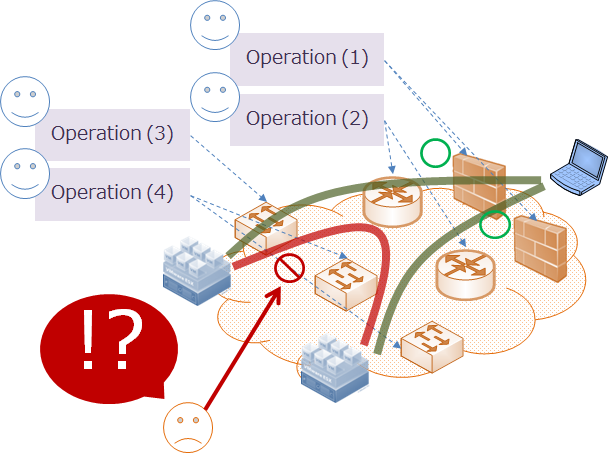
\includegraphics[scale=0.5]{img/difficulty-of-network-operation.png}
  \caption{ネットワーク全体の動作確認の難しさ}
  \label{fig:difficulty-of-network-operation}
 \end{figure}

ネットワーク全体としての動作保証の難しさは以下のような要素に起因すると考
えられる。
\begin{itemize}
 \item ネットワークでは機器それぞれが様々なポリシをもとにトラフィックを
       制御する。それらは周囲の機器と交換される制御情報、実際にながれて
       いるその時々のトラフィックなどにも影響される。
 \item ネットワーク全体の動作は隣接する機器間で相互に設定情報の整合性を
       とる必要があり、使用している機器や技術の数が増加するほど検討すべ
       き組み合わせのパターンが増大する。
 \item ネットワークは、そのリソースを通常複数のシステムやユーザで共有す
       る。システムの上流ネットワークほど共有度が高くなり、機能変更や障
       害時の影響範囲が広くなる。
 \item ネットワークは状態に応じて動作が変化する。ネットワークの状態とし
       ては、機器内部でキャッシュされる転送制御情報・発生した通信のセッ
       ションやコネクションの情報といった機器単体の状態、物理リンク増減・
       トポロジのようになネットワーク全体の状態がある。ネットワーク全体
       としての動作は、こうしたさまざまな状態に応じて変化するため、同一
       のイベントに対して常に一定の動作がおこなわれるとは限らない。
\end{itemize}

こうした理由から、大規模なネットワークや、仮想化技術などをつかった複雑性・
共有度が高くかつ動的な構成変更がおこなわれるネットワークでは、ネットワー
クに対する設定変更・構成変更の影響範囲を正確に判断することは非常に難しく
なっている。

  \section{従来のネットワークテストとネットワークテストに着目する理由}

  % 運用の理想像や現状
  % TODO: ITHD技術交流会資料
  % \url{https://drive.google.com/drive/folders/0B2eRR_JxYJA5OFkzUFlveVlObWc}
  % p6-7 あたりとかの話をいれる

ネットワークの構築や運用では、自動化の難しさや設定変更による影響範囲の予
測のしにくさなどの課題がある(\ref{sec:system-problem}節)。こうした課題に
より、従来のネットワーク(特に高いサービスレベルが要求されるシステムのネッ
トワーク)の構築・運用では以下のような状況がみられる。
\begin{itemize}
 \item ネットワークの構成変更を実施する際は、その物理構成操作の要求やト
       ラブル発生時の現地対応リスクなどを加味して、特定の場所に人や端末
       を配置しながら人手でテストを実行していくという、人海戦術的オペレー
       ションをとる。
 \item 特定の設定変更によってどの程度のサービス影響があるのか判断するこ
       とが難しいため、機器やサービスの知見者を集めて、変更した場合の影
       響検討をくりかえしおこなう。(複数回のレビューを実施する。)
\end{itemize}
いずれにせよ、これらは現地・現物・人海戦術的なやりかたとなる傾向があり、
システム(サービス)にもとめられる迅速性(agility)を落とすボトルネックにな
りがちである。

影響範囲予測の難しさへの対策として、検証環境を用意して、そこで実際に想定
されるオペレーションを実行することもおこなわれる。しかし、ネットワーク規
模や構成の大規模化・複雑化とそれによるテストパターン数の増大にともない、
テストパターンをすべて人手で網羅することは非常に難しい。そのため次のよう
な状況(リスク)を受け入れざるをえない。
\begin{description}
 \item[テスト作業用リソースの確保] 通常、テストをおこなうための人・機器
            の準備には制約がある。人手による作業の場合、作業コスト・時間
            や規模がどうしてもスケールさせられないため、小規模なオペレー
            ションで は十分なテストができないまま本番環境での作業になる
            傾向がある。
 \item[本番環境と検証環境の差分] リソース確保の都合、多くの場合では検証
            環境と本番環境では使用する機材や構成などに違いがある
            \footnote{同一製品ラインだがスペック・ライセンスの異なるもの
            を使う、あるいは仮想アプライアンス版で検証をおこなう、などが
            検証環境での選択肢としてあるが、特定の機器や機能の組み合わせ、
            特定のハードウェアやソフトウェアでのみ発生するトラブルなども
            ある。}。また、実際にネットワーク内部を流れるトラフィックな
            どを再現するのは非常に難しい\footnote{特に非機能要件、性能や
            可用性要件などを検証環境で保証することは難しい。環境を段階的
            に拡張した結果として性能問題がおきる、特定の利用者による過負
            荷によりトラブルがおきるなど、事前・別環境での再現が難しい問
            題がある。}。そのため、検証環境では発生しなかった問題やトラ
            ブル、影響の見落としが本番環境の作業で初めて現れることがある。
 \item[代表パターンのみのテスト] 代表例のピックアップ(サンプリング)をし
            たテストケースでは、どうしてもサンプリングからもれた一部の設
            定ミスや不整合などを見落とすリスクがある。
 \item[テスト結果判断のばらつき] 手順書の解釈、操作の実行や結果の取得・
            判断などがテスト実行者に依存するため、本来問題となる事象を見
            落としてしまうリスクがある。これに加えて、複数人でテストを実
            行している場合は、個別に取得した情報を統合してネットワーク全
            体としての動作を判断しなければならないというオーバーヘッドが
            発生する。
\end{description}

%%% Local Variables:
%%% mode: yatex
%%% TeX-master: "main.tex"
%%% End:
